\begin{center}
     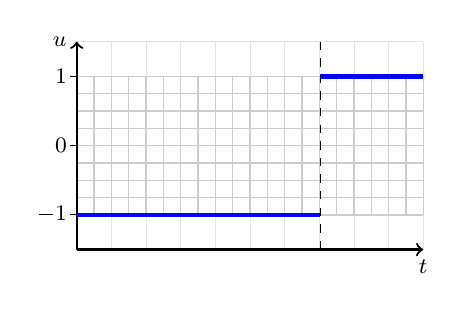
\begin{tikzpicture}[scale=0.88]
       \draw[draw=black!10,line width=0.25] (0,-1.5) grid[step=0.5] (5,1.5);
       \draw[draw=black!20,line width=0.5] (0,-1) grid[step=0.25] (5,1);
       \draw[thick,->] (0,-1.5) -- (5,-1.5) node[below] {\footnotesize{$t$}};
       \draw[thick,->] (0,-1.5) -- (0,1.5) node[left] {\footnotesize{$u$}};
       \foreach \u in {-1,0,1} {
         \draw (0,\u) node[left] {\footnotesize{$\u$}};
         \draw (-0.1,\u) -- (0,\u);
       }
       % Steuerung u
       \draw[ultra thick,blue] plot[domain=0:3.5174292] (\x,-1);
       \draw[ultra thick,blue] plot[domain=3.5174292:5] (\x,1);
       \draw[dashed] plot coordinates {(3.5174292,1.5) (3.5174292,-1.5)};
     \end{tikzpicture}
     %
     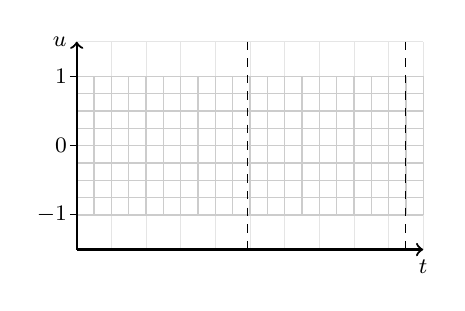
\begin{tikzpicture}[scale=0.88]
       \draw[draw=black!10,line width=0.25] (0,-1.5) grid[step=0.5] (5,1.5);
       \draw[draw=black!20,line width=0.5] (0,-1) grid[step=0.25] (5,1);
       \draw[thick,->] (0,-1.5) -- (5,-1.5) node[below] {\footnotesize{$t$}};
       \draw[thick,->] (0,-1.5) -- (0,1.5) node[left] {\footnotesize{$u$}};
       \foreach \u in {-1,0,1} {
         \draw (0,\u) node[left] {\footnotesize{$\u$}};
         \draw (-0.1,\u) -- (0,\u);
       }
       % Steuerung u
       \draw[blue,ultra thick] plot file {data/datenualpha.txt};
       \draw[dashed] plot coordinates {(2.4700,1.5) (2.4700,-1.5)};
       \draw[dashed] plot coordinates {(4.7500,1.5) (4.7500,-1.5)};
     \end{tikzpicture}
     \captionof{figure}{Optimale Steuerung f\"ur $\alpha = 0$ (links) und $\alpha = 1$ (rechts)}
\end{center}